\chapter{不等式与极限定理}

\section{概率不等式}

\begin{theorem}{Markov不等式}{Markov inequality}
	若随机变量$X\geqslant0$且期望有限，则$\forall\varepsilon>0$，有
	\begin{equation}
		\label{eqn:Markov ineq}
		\P(X\geqslant\varepsilon)\leqslant\frac{\E(X)}\varepsilon.
	\end{equation}
\end{theorem}

\begin{proof}
	引入示性函数(characteristic function)
	\begin{equation}
		1(X\in A):=\begin{cases}
			1,&X\in A\\
			0,&X\notin A
		\end{cases}
	\end{equation}
	则$1(X\geqslant\varepsilon)\leqslant X/\varepsilon$，两边取期望，即证。
\end{proof}

\begin{theorem}{Chebyshev不等式}{Chebyshev inequality}
	若随机变量$X$的方差$\Var(X)$存在，则$\forall\varepsilon>0$均有
	\begin{equation}
		\P(\abs{X-\E(X)}\geqslant\varepsilon)\leqslant\frac{\Var(X)}{\varepsilon^2}.
	\end{equation}
\end{theorem}

\begin{proof}
	由Markov不等式
	\[
		\P\bigb{\bigp{X-\E(X)}^2\geqslant\varepsilon^2}\leqslant\frac{\E\bigb{\bigp{X-\E(X)}^2}}{\varepsilon^2}\equiv\frac{\Var(X)}{\varepsilon^2}.
		\qedhere
	\]
\end{proof}

\begin{theorem}{Chernoff不等式}{Chernoff inequality}
	对随机变量$X$，$\forall\varepsilon>0,\forall t>0$使得$\E(\e^{tX})$存在，有
	\begin{equation}
		\P(X\geqslant\varepsilon)\leqslant\frac{\E(\e^{tX})}{\e^{t\varepsilon}}.
	\end{equation}
\end{theorem}

\begin{proof}
	由Markov不等式，
	\[
		\P(X\geqslant\varepsilon)=\P(\e^{tX}\geqslant\e^{t\varepsilon})\leqslant\frac{\E(\e^{tX})}{\e^{t\varepsilon}}.
		\qedhere
	\]
\end{proof}
\begin{remark}
	即使$X$矩母函数不存在，不等式也成立。
\end{remark}

\begin{example}{正态分布的尾概率估计}{}
	$X\sim\NormalDist(0,1)$，则三个不等式给出
	\[
		\P(\abs{X}\geqslant 3)\leqslant\begin{cases}
			\frac13\E(\abs X)=\frac13\sqrt{\frac2\pi}\doteq 0.27,&\text{(Markov)}\\[2ex]
			\frac19\Var(X)=\frac19\doteq 0.11,&\text{(Chebyshev)}\\[2ex]
			\inf_{t>0}2\e^{t^2/2-3t}=2\e^{-9/2}\doteq 0.022.&\text{(Chernoff)}
		\end{cases}
	\]
	比较而言，Markov仅用到了均值的信息，Chebyshev用到了方差的信息，Chernoff用到了各阶矩的信息。而结果也是越来越好的。
\end{example}

\begin{theorem}
	{Paley--Zygmund不等式}{Paley-Zygmund inequality}
	若随机变量$X\geqslant0$且$0<\E(X^2)<\infty$，则$\forall\lambda\in(0,1)$，有
	\begin{equation}
		\label{eqn:Paley-Zygmund ineq}
		\P(X\geqslant\lambda\E(X))\geqslant(1-\lambda)^2\frac{\E(X)^2}{\E(X^2)}.
	\end{equation}
\end{theorem}

\begin{proof}
	利用示性函数$1\equiv 1(X\in A)+1(X\in A\eventcomp)$：
	\begin{align*}
		\E(X)&=\E\bigb{X1\bigp{X\leqslant\lambda\E(X)}}+\E\bigb{X1\bigp{X>\lambda\E(X)}}\\
		&\leqslant\lambda\E(X)+\sqrt{\E(X^2)\P\bigp{X>\lambda\E(X)}}
	\end{align*}
	前者是自然的，后者是Cauchy--Schwarz不等式。移项即得。
\end{proof}

\section{大数定律}
为何能以某事件发生的频率作为该事件的概率的估计？
\begin{definition}{依概率收敛}{converge in probability}
	$X_1,X_2,\ldots$为随机变量序列，$X$为随机变量，若$\forall\varepsilon>0$，均有
	\[
		\lim_{n\to\infty}\P(\abs{X_n-X}\geqslant\varepsilon)=0,
	\]
	则称序列$X_n$依概率收敛(converge in probability)于$X$，记作
	\begin{equation}
		X_n\pto X.
	\end{equation}
\end{definition}
\begin{theorem}{Khinchin弱大数定律}{Khinchin WLLN}
	随机变量序列$X_1,X_2,\ldots$ iid，且$\E(X_i)=\mu$，则
	\begin{equation}
		\avg X_n:=\frac1n\sum_{i=1}^nX_i\pto\mu
	\end{equation}
	这就是Khinchin弱大数定律(weak law of large numbers, WLLN).\index{LLN, 大数定律}
\end{theorem}

\begin{corollary}
	% Khinchin LLN指出：
	数学期望可以由$n$个iid的随机变量的算术平均值近似。
\end{corollary}

\begin{remark}
	最初形式为Bernoulli LLN，应用于$X_i\sim\BernDist(p)$中用频率$\avg X$估计$p$。
\end{remark}

\begin{example}{用Chebyshev不等式证明Khinchin大数定律}{}
	若方差$\Var(X_i)=\sigma^2$存在\footnote{事实上Khinchin LLN并没有要求$\Var(X_i)$存在。}，则
	\begin{subequations}
		\begin{align}
			\E(\avg X_n)&=\frac1n\sum_{i=1}^n\E(X_i)=\mu,\\
			\Var(\avg X_n)&=\frac1{n^2}\sum_{i=1}^n\Var(X_i)=\frac{\sigma^2}n.
		\end{align}
	\end{subequations}
	由Chebyshev不等式
	\[
		\P(\abs{\avg X_n-\mu}\geqslant\varepsilon)\leqslant\frac{\sigma^2}{n\varepsilon^2}\to 0.
	\]
\end{example}

\begin{remark}
	Chebyshev LLN：$X_i$两两不相关，$\Var(X_i)$一致有界时，$\avg X_n-\E(\avg X_n)\pto0$。若各项均值为$\mu$，则$\avg X_n\pto\mu$。
\end{remark}

% 可对Kinchin LLN进行推广：当条件为，是；还有Markov LLN。

\begin{definition}{以概率1收敛}{converge almost surely}
	若随机变量序列$X_1,X_2,\ldots$极限存在，且
	\begin{equation}
		\P\Bigp{\lim_{n\to\infty}X_n=X}=1,
	\end{equation}
	则称序列$X_n$以概率1收敛(converge almost surely)于$X$，记作
	\begin{equation}
		X_n\asto X.
	\end{equation}
\end{definition}

\begin{corollary}
	以概率1收敛强于依概率收敛
\end{corollary}

\begin{example}{以概率1收敛强于依概率收敛}{}
	$\Omega=[0,1]$上的均匀分布，从而有$(\Omega,\eventspace,\P)$，定义
	\begin{align*}
		&Y_1(\omega)=I_{[0,1]}(\omega),\quad\omega\in[0,1]\\
		&Y_2(\omega)=I_{[0,1/2]}(\omega),\enspace Y_3(\omega)=I_{[1/2,1]}(\omega),\\
		&Y_4(\omega)=I_{[0,1/3]}(\omega),\enspace Y_5(\omega)=I_{[1/3,2/3]}(\omega),\enspace Y_6(\omega)=I_{[2/3,1]}(\omega),\\
		&\cdots
	\end{align*}
	显然，$Y_n$依概率收敛到0：
	\[
		\lim_{n\to\infty}\P(\abs{Y_n}\geqslant\varepsilon)=0.
	\]
	但$\lim_{n\to\infty}Y_n$不存在（总有破坏的区间），也就不存在以概率1收敛。
\end{example}

\begin{theorem}{Kolmogorov强大数定律}{Kolmogorov SLLN}
	若$X_1,X_2,\ldots$ iid，$\E(X_i)=\mu$，则
	\begin{equation}
		\avg X_n\asto\mu.
	\end{equation}
	即Kolmogorov强大数定律(\sout{powerful number law}, strong law of large numbers, SLLN).
\end{theorem}

\begin{remark}
	可见Kolmogorov SLLN和Khinchin WLLN条件相同且SLLN给出了更强的结论。
	但是这并不代表WLLN无用，在其他条件下，还会有其他形式的WLLN。
\end{remark}

\begin{corollary}
	概率的频率解释是合理的。这也是Monte Carlo积分原理的基础。
\end{corollary}

\section{中心极限定理}

\begin{definition}
	{依分布收敛}{converge in distribution}
	记$\CDF_n(x)=\P(X_n\leqslant x)$，$\CDF$为随机变量$X$的分布函数。若在$\CDF$的每个连续点$x$都有
	\[
		\lim_{n\to\infty}\CDF_n(x)=\CDF(x),
	\]
	则称$X_n$依分布收敛于$X$，记作
	\begin{equation}
		X_n\dto X.
	\end{equation}
\end{definition}

\begin{theorem}{Lindeberg--Lévy中心极限定理}{Lindberg-Levi CLT}
	随机变量序列$X_1, X_2,\ldots$ iid，且期望为$\mu$，方差满足$0<\sigma^2<\infty$。$\avg X$的标准化变量$Z_n$依分布收敛于标准正态分布$\NormalDist(0,1)$：
	\begin{equation}
		Z_n:=\frac{\avg X-\mu}{\sigma/\!\sqrt n}%\equiv\sum_{i=1}^n\frac{X_i-\mu}{\sqrt n\sigma}
		\dto Z\sim\NormalDist(0,1).
	\end{equation}
	称为Lindeberg--Lévy中心极限定理(central limit theorem, CLT)。\index{CLT, 中心极限定理}
\end{theorem}
\begin{proof}
	标准正态分布的CF $\CF(t)=\e^{-t^2/2}$，%不失一般性(without loss of generality, WLOG)，
	\begin{align*}
		\CF_{Z_n}(t)&=\biggb{\CF_{X_i-\mu}\biggp{\frac{t}{\sqrt n\sigma}}}^n\\
		&=\biggp{1+0+\frac12\CF''_{X_i-\mu}(0)\cdot\biggp{\frac{t}{\sqrt n\sigma}}^2+o\biggp{\frac{t^2}n}}^n\\
		&=\biggp{1-\frac{t^2}{2n}+o\biggp{\frac{t^2}n}}^n\to\e^{-t^2/2}.
		\qedhere
	\end{align*}
\end{proof}

\begin{corollary}
	我们可以近似的认为$\avg X\dotsim\NormalDist(\mu,\sigma^2/n)$。
\end{corollary}

\begin{example}{de Moivre--Laplace中心极限定理}{DeMoivre-Laplace CLT}
	特别地，若$X_i$独立同分布于$\BernDist(p)$且$0<p<1$，则二项变量$Y_n:=X_1+\cdots+X_n$满足$(Y_n-np)/\sqrt{np(1-p)}\dto\NormalDist(0,1)$。因此大样本下有
	\[
		\P(Y_n\leqslant t)\doteq\Phi\biggp{\frac{t-np}{\sqrt{np(1-p)}}}.
	\]
	\begin{notecaptionblock}
		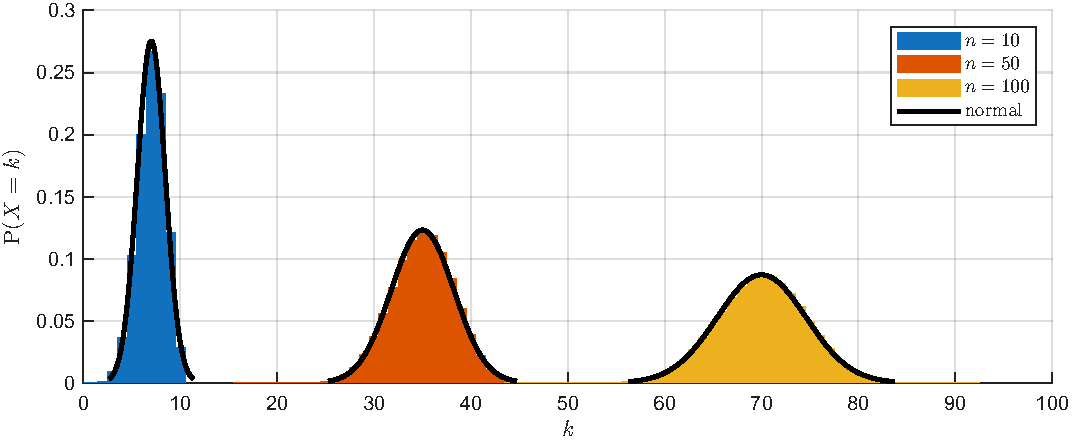
\includegraphics[width=0.9\linewidth]{figures/CLT_bin.pdf}
		\captionof{figure}{二项分布的CLT近似}
		\label{fig:CLT_bin}
	\end{notecaptionblock}
	对整数端点$t_1,t_2$作连续性修正，得到
	\[
		\P(t_1\leqslant Y_n\leqslant t_2)\doteq\Phi\biggp{\frac{t_2-np+1/2}{\sqrt{np(1-p)}}}-\Phi\biggp{\frac{t_1-np-1/2}{\sqrt{np(1-p)}}}.
	\]
	这称为de Moivre--Laplace CLT。
\end{example}
\begin{example}{选举问题}{}
	为统计选民支持度$p$ （未知），随机调查$n$个人，支持比例$P_n=\avg X$，$N\gg n$近似的，可视为有放回$X_i\sim\BernDist(p)$，且
	\[
		\frac{P_n-p}{\sqrt{p(1-p)/n}}\dotsim\NormalDist(0,1)
	\]
	要求精度$\varepsilon=0.03$，置信度为\qty{95}{\percent} ($\alpha=0.05$)，CLT给出
	\[
		\P(\abs{P_n-p}\geqslant\varepsilon)\doteq 2\biggb{1-\Phi\biggp{\frac\varepsilon{\sqrt{p(1-p)/n}}}}\leqslant\alpha
	\]
	当$p=1/2$时$n_{\min}$最大：
	\[
		n_{\min}=\left\lceil\biggp{\frac{\Phi^{-1}(1-\alpha/2)}{2\varepsilon}}^2\right\rceil=1068.
	\]%1.96
	与$N$无关。
	这说明只需要调查一千多人，就可以以\qty{95}{\percent}的置信度估计选民支持度$p$在$P_n\pm 0.03$的范围内。
\end{example}
\begin{theorem}{Lyapunov中心极限定理}{Lyapunov CLT}
	随机变量序列$X_1,X_2,\ldots$是独立的随机变量序列，且具有期望和方差
	\[
		\E(X_k)=\mu_k,\quad\Var(X_k)=\sigma_k^2;\quad B_n^2:=\sum_{k=1}^n\sigma_k^2.
	\]
	若存在$\delta>0$满足Lyapunov条件：
	\[
		\lim_{n\to\infty}\frac1{B_n^{2+\delta}}\sum_{k=1}^n\E\bigp{\abs{X_k-\mu_k}^{2+\delta}}=0.
	\]
	则随机变量之和的标准化变量依分布收敛于标准正态分布：
	\begin{equation}
		\label{eqn:Lyapunov CLT}
		Z_n:=\frac1{B_n}\sum_{k=1}^n(X_k-\mu_k)\dto Z\sim\NormalDist(0,1).
	\end{equation}
\end{theorem}
这说明，当$N$很大时，
\begin{equation}
	\sum_{i=1}^nX_i\dotsim\NormalDist\biggp{\sum_{i=1}^n\mu_i,\sum_{i=1}^n\sigma_i^2}.
\end{equation}

\begin{theorem}{Markov中心极限定理}{Markov CLT}
	设有限状态、不可约、非周期的时齐Markov链$S_i$从平稳分布$\pi$出发，$X_i=f(S_i)$为实值观测。记$\mu=\E_\pi(X_i)$和$\gamma_k=\Cov_\pi(X_1,X_{1+k})$，则长期方差为
	\[
		\sigma_{\mathrm L}^2=\gamma_0+2\sum_{k=1}^\infty\gamma_k .
	\]
	在上述条件下协方差级数绝对收敛。若$\sigma_{\mathrm L}^2>0$，则
	\begin{equation}
		\label{eqn:Markov CLT}
		\frac{\sqrt n(\avg X_n-\mu)}{\sigma_{\mathrm L}}\dto\NormalDist(0,1).
	\end{equation}
\end{theorem}

\begin{remark}
	总结：
	\begin{compactenum}
		\item 尾部概率控制；
		\item LLN, CLT；
		\item CLT的应用：$\avg X\dotsim\NormalDist(\mu,\sigma^2/n),\enspace\sum\nolimits_{i=1}^nX_i\dotsim\NormalDist(n\mu,n\sigma^2)$；
		\item 三种收敛：$\asto,\pto,\dto$。
	\end{compactenum}
\end{remark}